\section{NNPDF Monte Carlo approach to inverse problems}
\label{sec:closure-test}

In this section we discuss the NNPDF approach to inverse problems, and make
contact explicitly with the formalism laid out in
Sec.~\ref{sec:inverse-problems}. In the Bayesian formulation,
Eq.~\ref{eq:PosteriorModel} gives a quantitative description of how the
information contained in the experimental data propagates into our knowledge of
the space of models. In practice, it should be possible to sample directly from
the posterior distribution, or to find a solution using some kind of
Backus-Gilbert methodology~\cite{BackusGilbert1968}. These new types of approach
are not straightforward and we defer their investigation to further, dedicated
studies. Here we focus instead on the standard NNPDF fitting procedure and
investigate its relation with the Bayesian result. The NNPDF approach generates
an ensemble of fit results, which are supposed to describe the posterior
probability distribution for the model (\ie\ in the space of PDFs) given the
experimental data. In the case of a linear map, we show here that this is
exactly the case: the NNPDF replicas are distributed exactly accroding to the
posterior density that was obtained in the previous section. 

\subsection{Fitting replicas}
\label{sec:fit-reps}

The approach for generating a sample in model space utilised by NNPDF can
broadly be described as fitting model replicas to pseudo-data replicas. As
discussed in Eq.~\ref{eq:NoisyInverseProblem} the experimental values are
subject to observational noise. If we assume this observational noise to be
multigaussian then the experimental central values, $\obspriorcent$, are given
explicitly by
\begin{equation}
    \label{eq:levelonedata}
    \obspriorcent = \law + \obsnoise,
\end{equation}
where $\law$ is the vector of {\em true} observable values, and the
observational noise is drawn from a Gaussian centred on zero such as in
Eq.~\ref{eq:RhoGauss}, \ie\ $\obsnoise \sim \mathcal{N}(0, \obspriorcov)$ where
$\obspriorcov$ is the experimental covariance matrix. In
Eq.~\ref{eq:levelonedata}, each basis vector corresponds to a separate data
point, and the vector of shifts $\obsnoise$ permits correlations between data
points according to the covariance matrix provided by the experiments. Given the
data, the NNPDF approach is to compute a MAP estimator along the lines discussed
in the previous section, \ie\ finding the model that minimises the $\chi^2$ to
the data.~\footnote{In order to avoid overfitting, the NNPDF fitting procedure does 
not aim for the absolute minimum of the $\chi^2$ defined from the training sample. 
Instead a conventional split between training and validation is used. The details 
of this procedure are not relevant for the current discussion and will be neglected here.} 
The key difference between the NNPDF approach and the classical MAP
estimator is that instead of fitting the observational data given by
Eq.~\ref{eq:levelonedata}, an ensemble of model replicas are fitted each to an
independently sampled instance of pseudo-data, which is generated by augmenting
$\obspriorcent$ with some noise, $\noise^{\repind}$,
\begin{equation}
    \label{eq:leveltwodata1}
    \pseudodat^{\repind} = \obspriorcent + \noise^{\repind}
    = \law + \obsnoise + \noise^{\repind},
\end{equation}
where $k$ is the replica index and each instance of the noise, $\noise$, is
drawn independently from the same Gaussian from which the observational noise is
drawn from, \ie\ $\noise \sim \mathcal{N}(0, \obspriorcov)$. For each replica
$k$, $\pseudodat^{\repind}$ is a vector in $\real^{\ndata}$. The distribution of
pseudo-data in a simple one-dimensional example is shown in
Fig.~\ref{fig:DistRep}. Note that, if we were to repeat this construction
multiple times, the true value $f$ would be within a 1$\sigma$ interval centred
at $y_0$ with a 68\% probability.
\begin{figure}
    \centering
    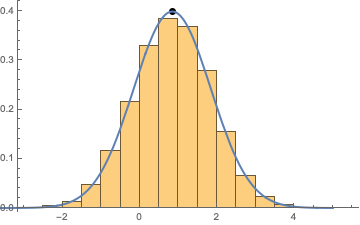
\includegraphics[scale=0.8]{ReplicaDistribution.png}
    \caption{Histogram showing the distribution of $10^4$ replicas generated
    around an experimental value $y_0$ with unit variance. The central value
    $y_0$, which is represented by the solid dot at the centre of the replica
    distribution, is drawn from a Gaussian distribution with unit variance
    centred at the true value $f$, which is assumed to be the origin in this
    plot. The central value $y_0$ is kept fixed for the whole set of
    replicas.\label{fig:DistRep}}
\end{figure}

The parameters for each model replica maximise the likelihood evaluated on the
corresponding pseudo-data. We can think of this approach as a special case of
MAP estimation, as described in Eq.~\ref{eq:MAP}, where there is no model
prior that regulates the likelihood. Another way of viewing this is to take
$\modelpriorcov^{-1} \to 0$ in Eq.~\ref{eq:MAP}, as was done to obtain the
result in Eq.~\ref{eq:NoPriorLinModel}. Either way, there is no prior
information about the model. The parameterisation of the model is fixed, so the
model space is the space of parameters $\modelvec \in \real^{\nmodel}$. In
$\real^{\nmodel}$, we find the parameters which minimise the $\chi^2$ between
the predictions from the model and the corresponding pseudo-data
$\pseudodat^{\repind}$
\begin{equation}\label{eq:NNPDFLikelihood}
    \begin{split}
        \modelvecrep &= \arg\min_{\modelvec^{\repind}} \repchis \\
        &= \arg\min_{\modelvec^{\repind}} \sum_{ij}
        \left( \fwdobsop(\modelvec^{\repind}) - \pseudodat^{\repind} \right)^T
        \obspriorcov^{-1}
        \left( \fwdobsop(\modelvec^{\repind}) - \pseudodat^{\repind} \right) \, ,
    \end{split}
\end{equation}
where, as usual, minimising the $\chi^2$ is equivalent to maximising the
likelihood, $\likelihood$, since $\chi^2 \equiv -\log{\likelihood}$.

As a final note: since we do not include the model prior, overall normalisations
can be omitted in Eq.~\ref{eq:NNPDFLikelihood}. It is clear however that if we
were including a model prior in our MAP, it is important that the relative
normalisation between the likelihood function and the model prior is clearly
specified.

\subsection{Fluctuations of fitted values}
\label{sec:fluct-fit-values}

It is not immediately obvious that the MC methodology, maximising the likelihood
on an ensemble of pseudo-data replicas, guarantees that the model replicas are
indeed sampled from the posterior distribution of parameters given data as
described \eg\ in Eq.~\ref{eq:PosteriorModel}. In order to investigate this
issue, we will again consider a model whose predictions are linear in the model
parameters, so that the posterior distribution of model parameters can be
computed explicitly. DIS observables can be seen as an example of a linear
model. Let us assume that the PDF are parametrized by their values at selected
values of $x_i$, so that $u$ is a finite-dimensional vector 
\begin{equation}
    \label{eq:Uvector}
    u_i = u(x_i)\, , \quad i = 1, \ldots, \nmodel\, .    
\end{equation}
The observables are then computed by taking a matrix-vector multiplication of
the vector $u$ by a $\ndata \times \nmodel$ matrix, $F_{ij}$, which is called FK
table in the NNPDF jargon, 
\begin{equation}
    \label{eq:FKTabLinVec}
    y_i = \sum_{j=1}^{\nmodel} F_{ij} u_j\, ,
\end{equation}
where $i=1,\ldots,\ndata$. In this case the forward map coincides exactly with
the FK table, $\linmap_{ij} = F_{ij}$ and the sum in Eq.~\ref{eq:FKTabLinVec}
approximates the convolution in Eq.~\ref{eq:DISExample}. However it should be
clear that the discussion below applies to any model whose forward map can be
approximated as Eq.~\ref{eq:FKTabLinVec}, like a linear approximation of
neural networks~\cite{ADVANI2020428}. Let us consider for instance the actual
NNPDF parametrization, where the value of the PDF is given by a neural network
whose state is determined by a set of weights $\theta$. In this case $X$ is the
space of weights, the model will be specified by a vector $\theta$ in the space
of weights, and we are going to continue using $u$ to denote the PDF, so that 
\begin{equation}
    \label{eq:WeightsParam}
    u_i = u(x_i; \theta)\, .
\end{equation}
If the parameters have a sufficiently narrow distribution around some value
$\bar\theta$, then we can expand the expression for the observables:
\begin{align}
    y_i  &= 
        \sum_j F_{ij} \left[u(x_j; \bar\theta)
         + \sum_k \left.\frac{\partial u}{\partial \theta_k}\right|_{x_j,\bar\theta} 
         \left(\theta - \bar\theta\right)_k
        \right]
\end{align}
and therefore
\begin{align}
    y_i - \bar{y}_i &=
         \sum_k \linmap_{ik} \Delta\theta_k
        \,,         
\end{align}
where 
\begin{align}
    \linmap_{ik} &= 
        \sum_j F_{ij} \left.\frac{\partial u}{\partial \theta_k}\right|_{x_j,\bar\theta}\, , \\
    \bar{y}_i &= \sum_j F_{ij} u(x_j; \bar\theta)\, , \\
    \Delta\theta_k &= \theta_k - \bar\theta_k\, .
\end{align}

In order to get an exact analytical solution for the linear model, we
additionally require $\linmap$ to have linearly independent rows, and therefore
$\linmap \obspriorcov \linmap^T$ is invertible. As discussed in
Sec.~\ref{sec:inverse-problems}, in the absence of prior information on the
model, the posterior distribution of model parameters is a Gaussian with mean
and covariance given by Eqs.~\ref{eq:NoPriorLinModel} and
\ref{eq:NoPriorLinModelCov}.

Let us now stick to the parametrization in Eq.~\ref{eq:Uvector} and let us
deploy the NNPDF Monte Carlo method to fitting model replicas, then in the case
under study $\arg\min_{\modelvec^{\repind}} \repchis$ is found analytically by
imposing that the derivative of $\repchis$ with respect to the model parameters
is zero, i.e.
\begin{equation}
    \begin{split}
        \label{eq:MAPEstLinModel}
        \modelvecrep &= (\linmap^T \obspriorcov^{-1} \linmap)^{-1}
        \left(
            \linmap^T \obspriorcov^{-1} \obspriorcent +
            \linmap^T \obspriorcov^{-1} \noise^{\repind}
        \right) \, .
    \end{split}
\end{equation}
Eq.~\ref{eq:MAPEstLinModel} shows that $\modelvec_*$ is a linear combination of
the Gaussian variables $\noise$, and therefore is also a Gaussian variable. Its
probability density is then completely specified by the mean and covariance,
which can be calculated explicitly, given that the probability density for
$\noise$ is known:
\begin{align}
    \emodel{\modelvec_*} &=
    \modelpostcent = (\linmap^T \obspriorcov^{-1} \linmap)^{-1} \linmap^T
    \obspriorcov^{-1} \obspriorcent\, , \\
    {\rm cov}(\modelvec_*) &= \modelpostcov = (\linmap^T \obspriorcov^{-1} \linmap)^{-1} \, .
\end{align}
These two equations show that, under the assumptions specified above,
$\modelvec_* \sim \mathcal{N}(\modelpostcent, \, \modelpostcov)$. In other
words, when the model predictions are linear in the model parameters, the NNPDF
MC method is shown to produce a sample of models exactly distributed according
to the expected posterior distribution of model parameters given the data. When
we fit PDFs, parameterised as deep fully connected neural networks, to data
which includes hadronic observables, it is clear that the forward map is
non-linear, and therefore this proof does not strictly apply. As discussed
above, even for non-linear models we can make a linear approximation of the
forward map provided that we are expanding around the MAP estimator. This means
the NNPDF MC methodology should reproduce the posterior distribution of the
model given the data, at least close to $\modelpostcent$, the central value of
the fitted replicas. Furthermore, by fluctuating the data and fitting the
replicas, the fluctuations in data space are propagated to model space
non-linearly. So even for non-linear problems, the NNPDF MC methodology can be
expected to produce a sample of models which are at least approximately
distributed according to the posterior model distribution. It remains to be
shown, however, that further away from the MAP estimator the approximation holds
despite the non-linear dependence of the model replicas on the data
uncertainities.

\subsection{Closure test}
\label{sec:closure-test-intro}

The concept of the closure test, which was first introduced in
Ref.~\cite{nnpdf30}, is to construct artificial data by using a known
pre-existing function to generate the {\em true} observable values, $\law$. One
way of achieving this is by choosing a model $\lawmodel$ and then compute $\law
= \fwdobsop(\lawmodel)$. Then the experimental central values are artificially
generated according to Eq.~\ref{eq:levelonedata}, where the observational noise
is pseudo-randomly generated from the assumed distribution. In
Ref.~\cite{nnpdf30}, $\law$ is referred to as level 0 (L0) data and
$\obspriorcent$ is referred to as level 1 (L1) data. Finally, if we use the
NNPDF MC method to fit artificially generated closure data, the pseudo-data
replicas that are fitted by the model replicas are referred to as level 2 (L2)
data.

The outcome of the fit is then compared with the known {\em true} value to check
the precision and accuracy of the fitting procedure. Finding quantitative
estimators that allow us to characterise the quality of the closure fit is one
of the main problems that need to be addressed. We will discuss a new class of
estimators in the next section. 

Note that in a closure test, the assumed prior of the data is fully consistent
with the particular instance of observed central values, $\obspriorcent$: by
construction, there are no inconsistent data sets. In the original closure test
of Ref.~\cite{nnpdf30} there was also no modelisation uncertainty, the true
observable values were assumed to be obtained by applying the forward map
$\fwdobsop$ to a vector in model space $\lawmodel$. It is worth noting that the
assumption of zero modelisation uncertainties is quite strong and likely
unjustified in many areas of physics. In the context of fitting parton
distribution functions there are potentially missing higher order uncertainties
(MHOUs) from using fixed order perturbative calculations as part of the forward
map. MHOUs have been included in parton distribution fits \cite{NNPDF:2019vjt,
AbdulKhalek:2019ihb} and in the future these should be included in the closure
test, however this is beyond the scope of the study presented here, since MHOUs
are still not included in the NNPDF methodology by default. In the results
presented in the rest of this paper we do include nuclear and deuteron
uncertainties, as presented in \cite{Ball:2018twp, Ball:2020xqw, AbdulKhalek:2020yuc}, since they are
to be included in NNPDF fits by default. Extensive details for including
theoretical uncertainties, modelled as theoretical covariance matrices can be
found in those references. For the purpose of this study the modelisation
uncertainty is absorbed into the prior of the data, since
\begin{equation}
    \obspriorcent = \fwdobsop(\modelvec) + \obsnoise + \delta
\end{equation}
where $\delta \sim \mathcal{N}(0, \cov^{\rm theory})$. As long as the
modelisation uncertainty is independent of the data uncertainty, we can absorb
$\delta$ into $\obsnoise$ by modifying the data prior: $\obsnoise \sim
\mathcal{N}(0, C + C^{\rm theory})$. In doing that, we must also update the
likelihood of the data given the model to use the total covariance $(C + C^{\rm
theory})$. From now onwards we will omit $C^{\rm theory}$ because it is implicit
that we always sample and fit data using the total covariance matrix which
includes any modelisation uncertainty we currently take into account as part of
our methodology.

Mapping the closure test procedure to the quantities used in the Bayesian
treatment presented in the previous section will allow us to derive a number of
analytical results in Sec.~\ref{Sec:LinearMapEstimators}.
